\section{ANÁLISE DAS INSTALAÇÕES DO TCE-AM} % 296 lines

\hspace*{0.8cm}Este capítulo aborda as instalações do Tribunal de Contas do Estado do Amazonas, suas características de carga demandada e as máquinas de geração de energia que se encontram instaladas nas dependências do 

O objetivo desta análise foi adquirir as informações técnicas pertinentes ao funcionamento dos grupos geradores, suas especificações de conversão, a fim de estimar o potencial de geração de energia.

Com estes dados, foi possível analisar as possíveis adaptações necessárias para operar estes equipamentos utilizando o biodiesel como combustível.

A segunda parte do projeto consistiu no estudo das adaptações necessárias para que estes equipamentos possam operar utilizando o biodiesel como combustível, e, na sequência, a análise das implicações dessa mudança.

A unidade conta com um grupo gerador cuja potência aparente é de 750 kVA que atende os dois prédios principais, enquanto um segundo gerador, de potência aparente 450 kVA, atende o prédio anexo, que fica na parte de trás das dependências. 
    
\begin{figure}[H]
\begin{center}
			\caption{Entrada da subestação do TCE-AM}
			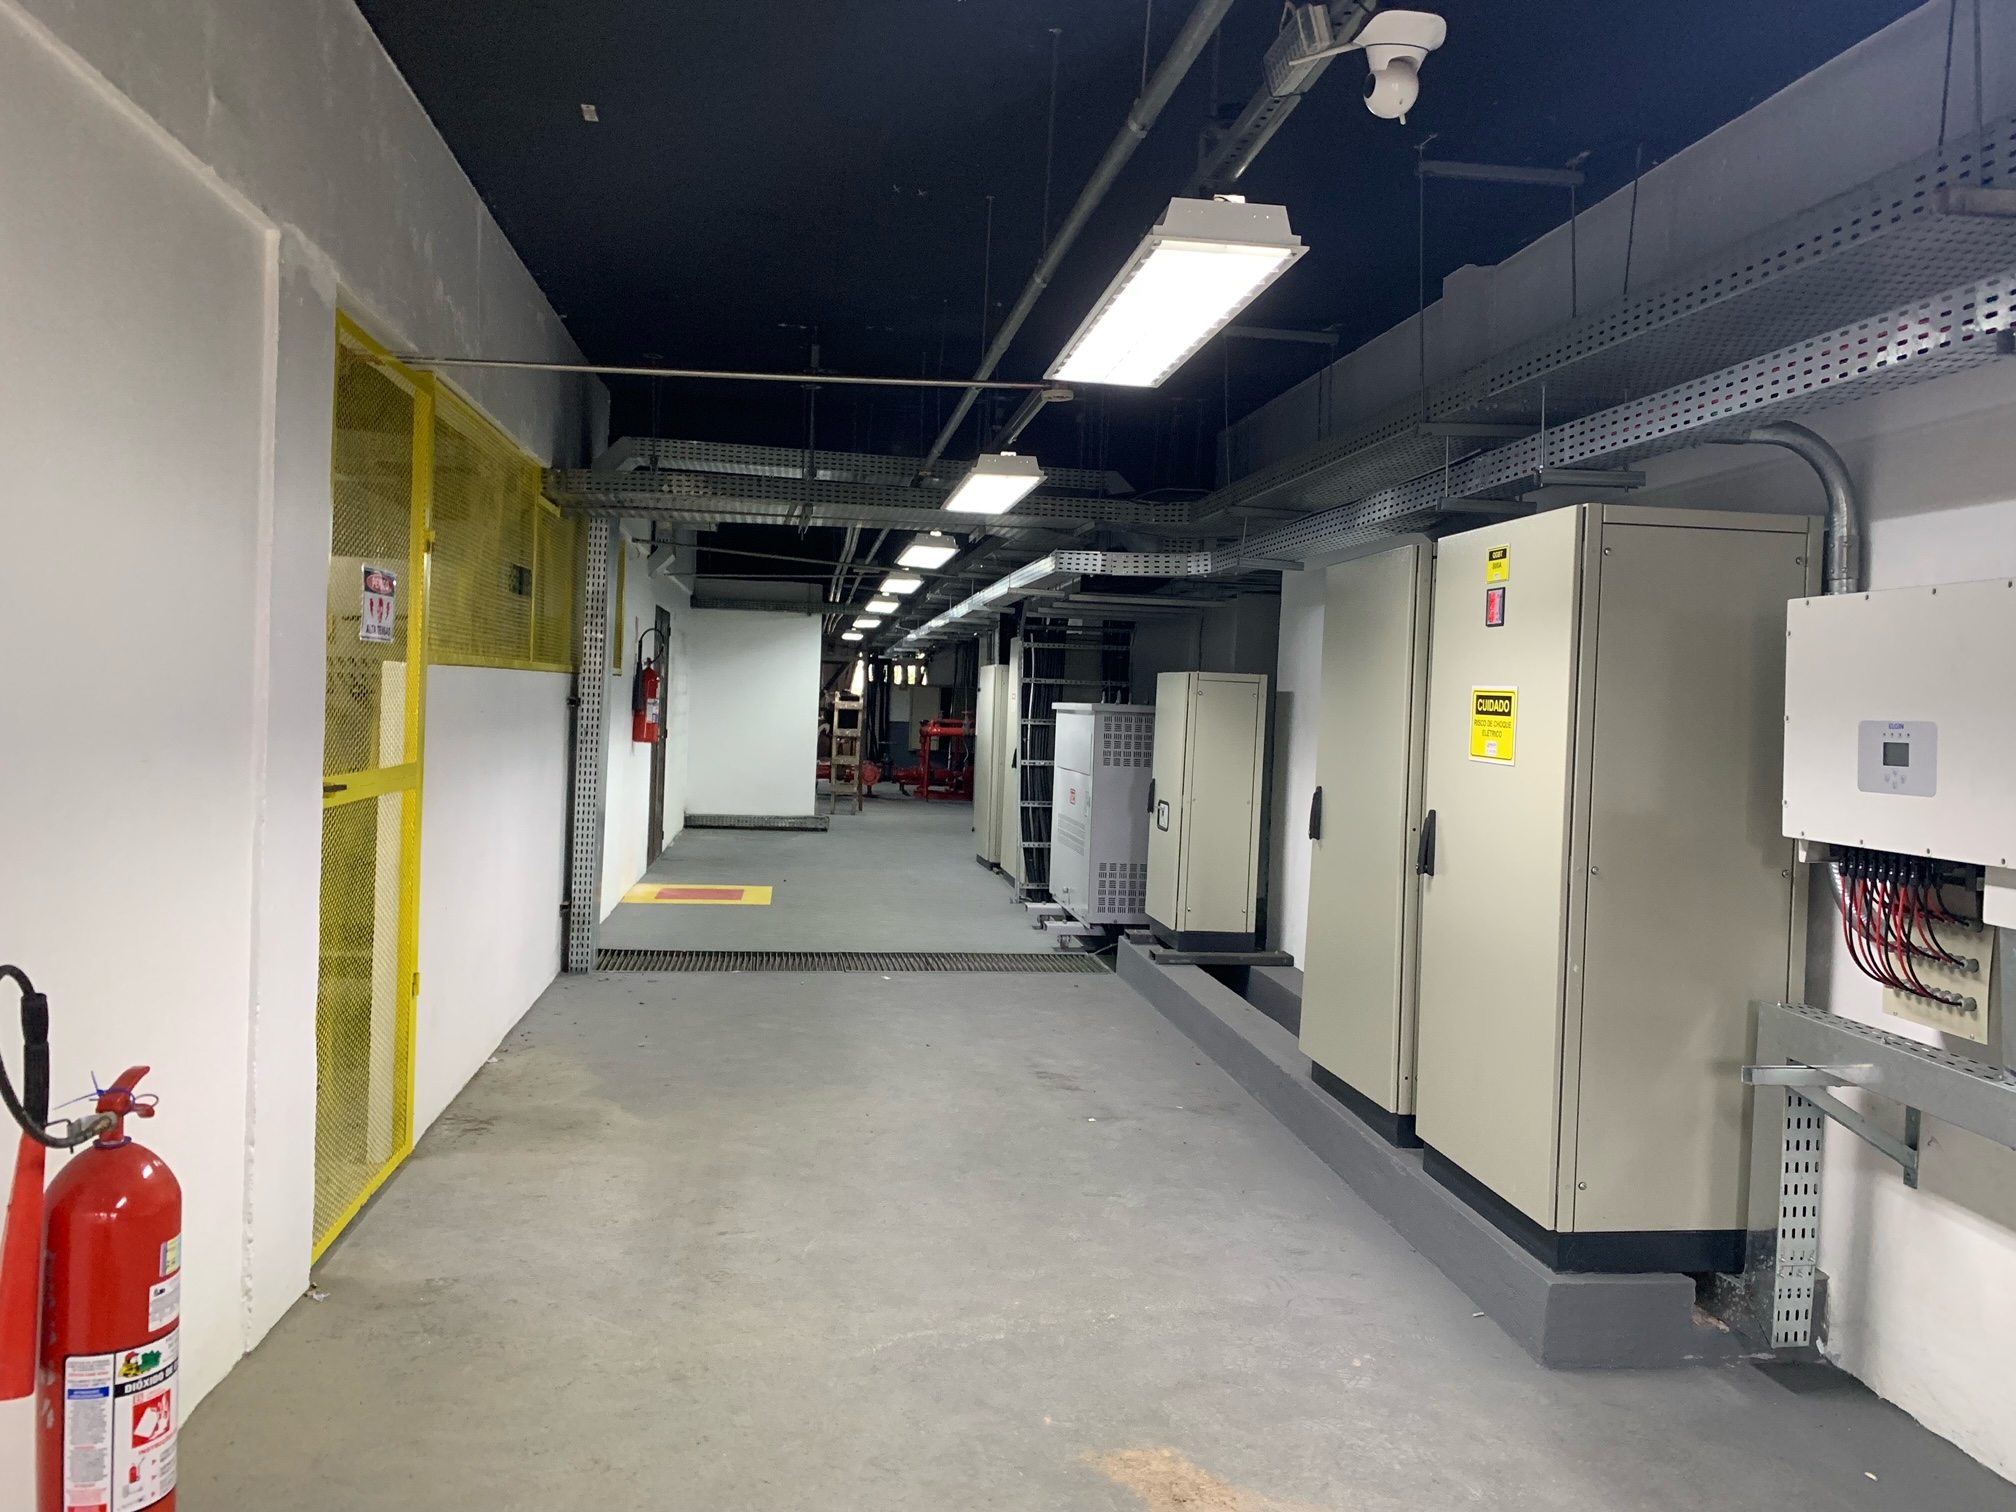
\includegraphics[width=.9\textwidth]{Figuras/deps.jpeg}
            \vspace*{\fill} 
            \begin{quote} 
            \centering 
            Fonte: própria.
            \end{quote}
            \vspace*{\fill}
			\label{fig:tceinst}
\end{center}
\end{figure}

Há, ainda, um terceiro grupo gerador, de 125 kVA, que atua somente como \textit{backup}, em caso de falha do primeiro. A razão para isto é que os prédios principais abrigam a Secretaria de Tecnologia da Informação (Setin), que conta com um Data Center, e este último gerador o alimenta exclusivamente.

A Figura \ref{fig:tceinst} mostra um panorama geral da subestação que se encontra no prédio principal e comporta o grupo gerador principal da unidade.

\subsection{Grupo gerador prédio principal}
\hspace*{0.8cm} O Grupo gerador principal (Figura \ref{fig:gerador750}) tem como responsabilidade atender os dois prédios principais da unidade. É importante resasltar que no momento da realização do estudo esse equipamento não atendia 100\% da unidade.

\begin{figure}[H]
\begin{center}
			\caption{Grupo gerador principal de 750 kVA}
			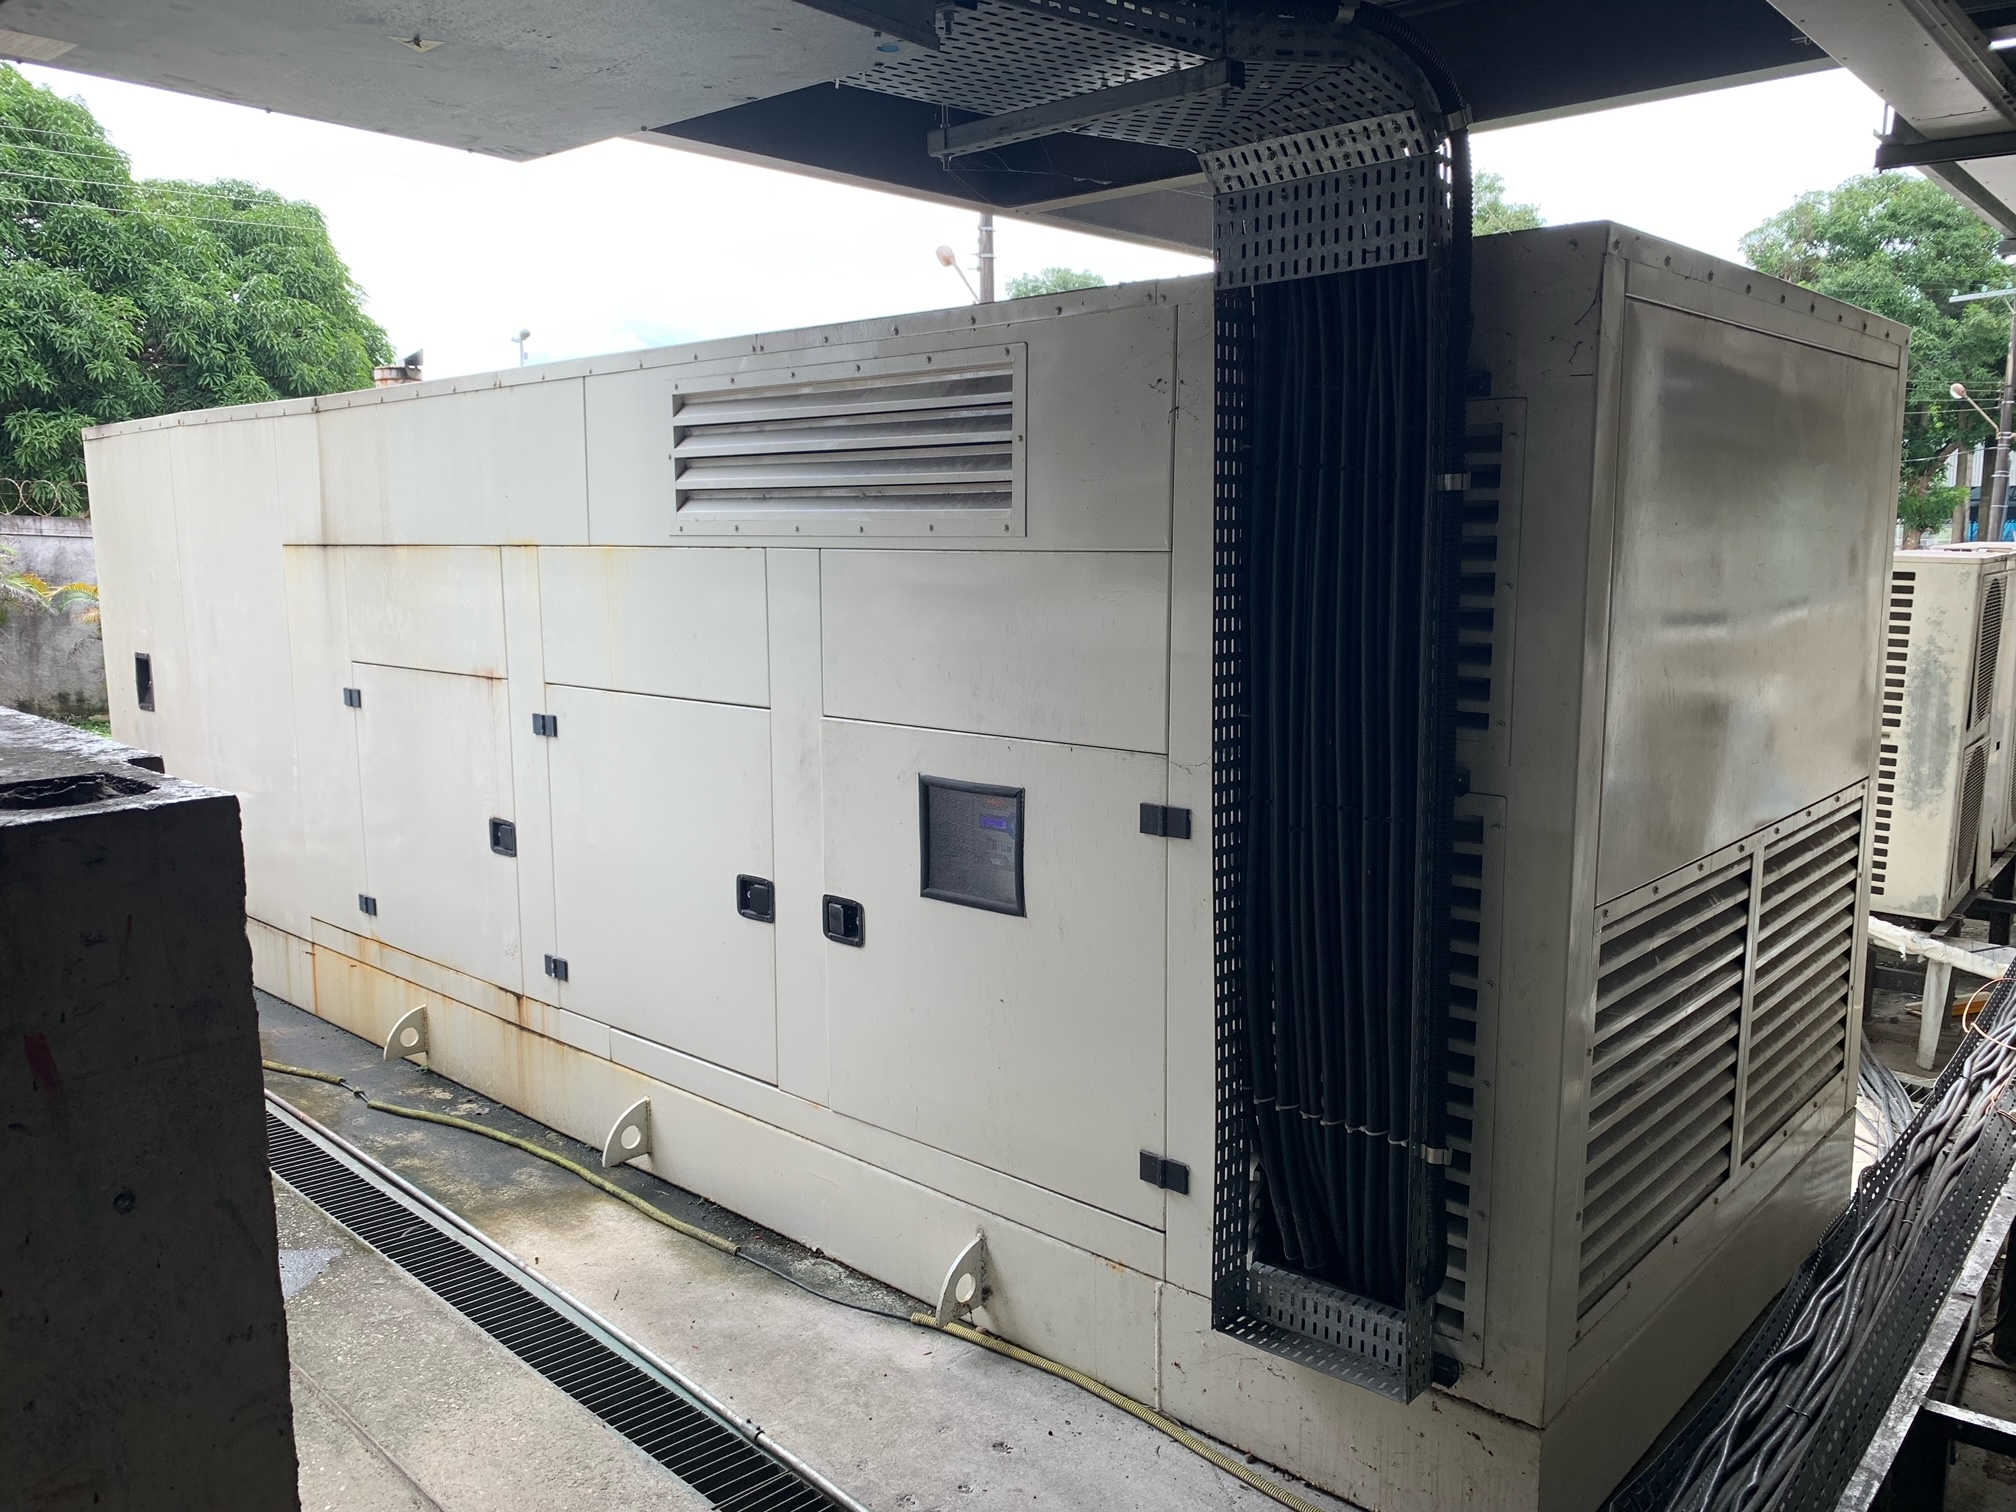
\includegraphics[width=.9\textwidth]{Figuras/gerador_750.jpeg}
            \vspace*{\fill} 
            \begin{quote} 
            \centering 
            Fonte: própria.
            \end{quote}
            \vspace*{\fill}
			\label{fig:gerador750}
\end{center}
\end{figure}

\subsubsection{Características de utilização}

\subsection{Grupo gerador prédio anexo}

\begin{figure}[H]
\begin{center}
			\caption{Grupo gerador prédio anexo de 450 kVA}
			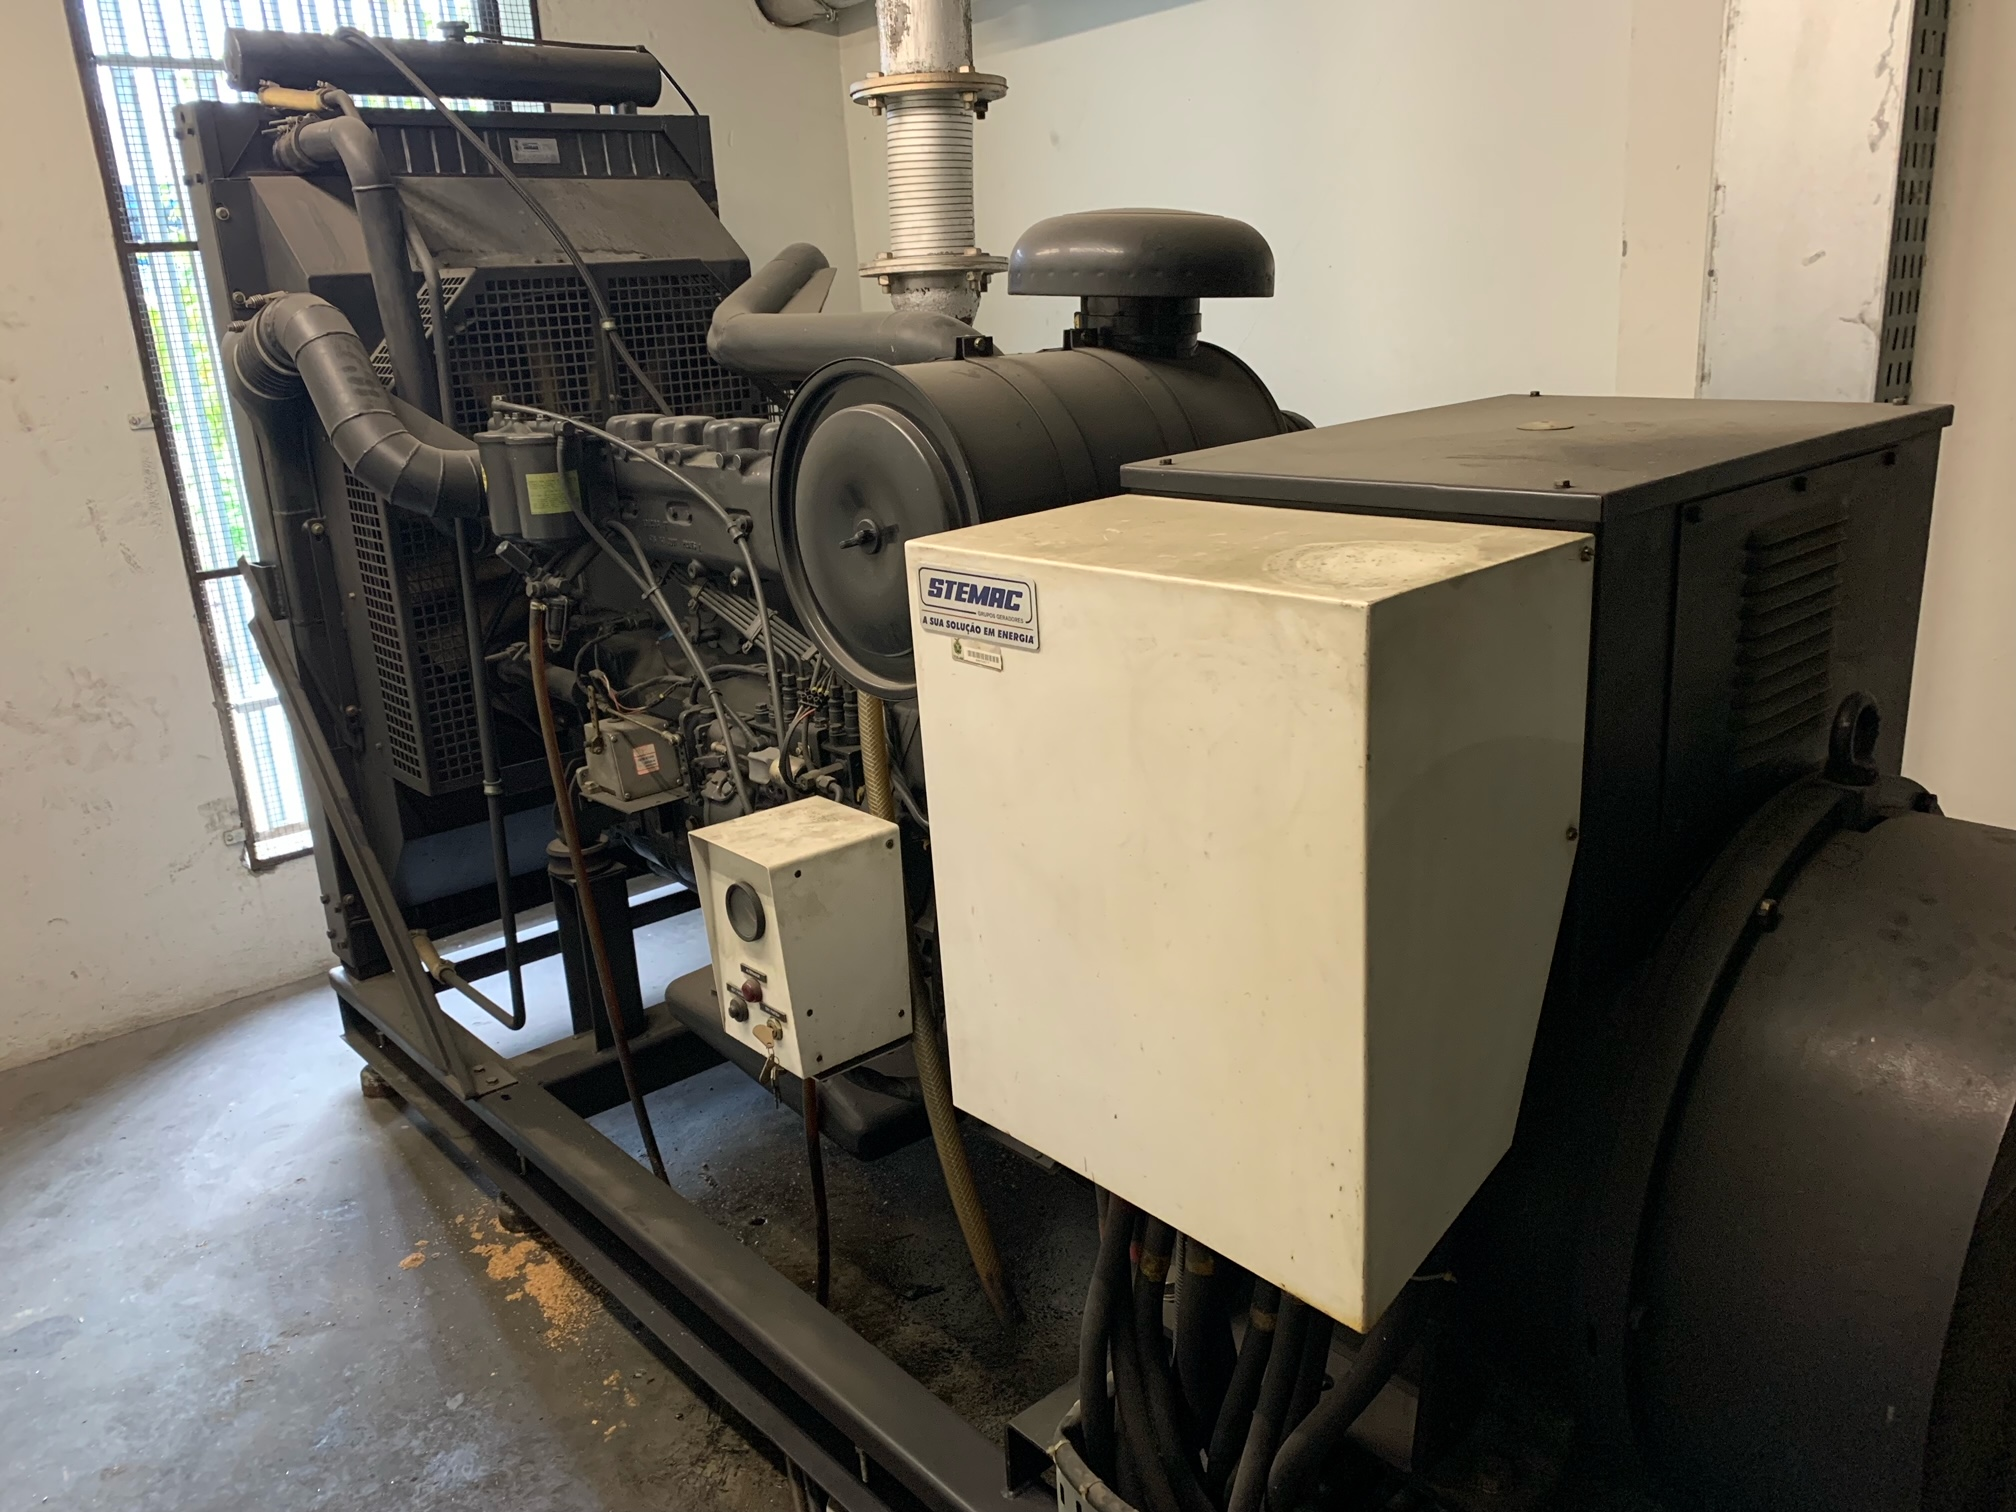
\includegraphics[width=.9\textwidth]{Figuras/gerador_450.jpeg}
            \vspace*{\fill} 
            \begin{quote} 
            \centering 
            Fonte: própria.
            \end{quote}
            \vspace*{\fill}
			\label{fig:gerador750}
\end{center}
\end{figure}
